\documentclass[11pt,a4paper]{article}
\usepackage[utf8]{inputenc}
\usepackage[T1]{fontenc}
\usepackage{lmodern}
\usepackage{hyperref}
\usepackage{url}
\usepackage{booktabs}
\usepackage{amsfonts}
\usepackage{graphicx}
\usepackage{tikz}
\usepackage{arxiv}
\usepackage{microtype}
\usepackage{float}

\title{The Ontology of the Alien:\\[0.5em]\large Escaping the Median Trap in LLM Ideation}
\def\shorttitle{The Ontology of the Alien}

\author{Henrik Westerberg\\Emergent Wisdom\\\texttt{henrik.westerberg@emergentwisdom.org}}

\date{March 2026\thanks{Revised April 2026. This revision integrates the Fractal Intelligence framework and makes the three-stage industrialization thesis explicit (\S\ref{sec:pipeline}), quantifies the structural-distinctness claim with sentence-embedding cosine similarity (\S3.1), clarifies the metacognition framing as functional rather than phenomenological (\S3.2), specifies the progressive-depth selection tournament, disambiguates `taxonomy' (the stored artifact) from `ontology' (the category-restructuring behavior), adds quantitative topology metrics (root count, depth, branching) to the graph-statistics table, includes verbatim four-phase traces of the Orthogonal Insight pipeline (\S2.4 and Appendix~\ref{sec:appendix-traces}), corrects several run-specific details against the dataset, and updates reference metadata. No new experiments were conducted. The original release remains archived at DOI~\href{https://doi.org/10.5281/zenodo.18912179}{10.5281/zenodo.18912179}.}}

\begin{document}
\maketitle

%%%%%%%%%%%%%%%%%%%%%%%%%%%%%%%%%%%%%%%%%%%%%%%%%%%%%%%%%%%%%%%%%%%%%%%%%%%%%%%
% ABSTRACT
%%%%%%%%%%%%%%%%%%%%%%%%%%%%%%%%%%%%%%%%%%%%%%%%%%%%%%%%%%%%%%%%%%%%%%%%%%%%%%%

\begin{abstract}
Large Language Models asked to ``be creative'' produce solutions that converge on a small number of archetypes---the Median Trap. We systematically compare eight methods for inducing structural diversity, contrasting simple prompting against three novel architectures: Semantic Tabu (accumulation of constraints), the Solution Taxonomy (a dual-agent ``Studio Model''), and the Orthogonal Insight Protocol (deriving mechanisms from alternative physics). In a controlled experiment ($N=196$), the Studio Model exhibited emergent metacognition: the system autonomously repaired its own taxonomy when faced with errors and actively commissioned research into unexplored conceptual regions. Under constraint pressure, the system synthesized novel combinations that do not emerge under standard prompting, including antifragility applied to gig-worker retirement (inverting risk flows so volatility benefits the system), metric dissolution (deconstructing problem variables), and ontological accommodation (restructuring categories when data defies classification). We release the method configurations and a dataset of 196 distinctly-labeled solution archetypes, demonstrating that adversarial ontological accommodation forces LLMs to escape the median.
\end{abstract}

\keywords{Artificial Intelligence, LLM Creativity, Cognitive Architecture, Prompt Engineering, Lateral Thinking, Multi-Agent Systems}

%%%%%%%%%%%%%%%%%%%%%%%%%%%%%%%%%%%%%%%%%%%%%%%%%%%%%%%%%%%%%%%%%%%%%%%%%%%%%%%
% INTRODUCTION
%%%%%%%%%%%%%%%%%%%%%%%%%%%%%%%%%%%%%%%%%%%%%%%%%%%%%%%%%%%%%%%%%%%%%%%%%%%%%%%

\section{Introduction: The Median Trap}

Ask a Large Language Model (LLM) to solve a difficult problem, and it will provide a reasonable answer. Ask it one hundred times, and it will provide one hundred variations of that same reasonable answer. This is the \emph{Median Trap}. Recent work confirms this pattern: when many users employ generative AI, individual outputs may improve while collective diversity collapses \cite{doshi2024}. Systematic benchmarking reveals the depth of the problem: only 0.28\% of LLM-generated responses reach the top 10\% of human creativity \cite{haase2025}, larger models within a family often exhibit \emph{less} diversity than their smaller counterparts \cite{zhang2025noveltybench}, and model size correlates negatively with epistemic diversity across topics and cultures \cite{wright2025}. Because LLMs minimize loss against training data, the past strictly dominates the future. The model's outputs collapse toward the average of what has already been said. Increasing the ``temperature'' parameter does not solve this; it merely adds lexical noise to the same underlying semantic structure, akin to shaking a camera rather than moving the photographer.

To generate genuinely non-obvious solutions, we must move the photographer. In prior work \cite{westerberg2025strangeworlds}, we introduced the Orthogonal Insight Protocol, a multi-agent pipeline that constructs coherent ``strange worlds'' with alternative physics and solves problems within them before extracting mechanisms back to reality. A controlled comparison showed that standard ``be creative'' prompting converges on five to six archetypes, while the protocol produces structurally diverse mechanisms. However, that study tested only one method against a baseline, leaving open the question of \emph{why} the protocol works and which components drive diversity.

This paper extends that work in three directions. First, we decompose the protocol into its constituent mechanisms and test them independently and in combination across eight conditions ($N=196$). Second, we introduce the Solution Taxonomy, a dual-agent ``Studio Model'' that exhibited self-directed behaviors not present in the original design. Third, we provide a comparative analysis showing how different constraint architectures shape not just the quantity of novel solutions but the topology of the resulting solution space.

%%%%%%%%%%%%%%%%%%%%%%%%%%%%%%%%%%%%%%%%%%%%%%%%%%%%%%%%%%%%%%%%%%%%%%%%%%%%%%%
% METHODS SECTION
%%%%%%%%%%%%%%%%%%%%%%%%%%%%%%%%%%%%%%%%%%%%%%%%%%%%%%%%%%%%%%%%%%%%%%%%%%%%%%%

\section{Methods}

We compare eight methods for inducing structural diversity in LLM ideation, organized by their inspiration source and novelty enforcement mechanism. To our knowledge, three are novel contributions (A, B, F), four are novel combinations (D, E, G, H), and one is an LLM operationalization of an established technique (C). Code and data are available via the experiment repository (\url{https://github.com/emergent-wisdom/ontology-of-the-alien}). All conditions address the same prompt: ``How do we build a retirement system for people who don't know how much they will earn next month, where `consistency' is impossible?'' We employed Claude Opus 4.5 for all experiments, targeting 25 solutions per condition (200 total). Conditions C--H utilized random seed words drawn from the Unix system dictionary (235,000 words). Due to incomplete negotiation in some taxonomy conditions, 196 solutions were ultimately generated (see Table~\ref{tab:solution-counts}).

\subsection{Condition A: Semantic Tabu}

Condition A relies on ``Semantic Tabu,'' where each solution is generated with full access to all previous solutions from the same run. This method enforces a strict three-step protocol: the model must first analyze previous solutions to extract mechanism-level features (rather than surface descriptions), then explicitly list the structural approaches it is avoiding, and finally generate a solution that evades all identified mechanisms. By the twenty-fifth run, the tabu list contains 24 distinct mechanism descriptions, forcing the model into increasingly unfamiliar territory. This approach directly applies Denial Prompting \cite{lu2025}, but with implementation-level refinements that enforce avoidance reasoning prior to generation and target deep semantic mechanisms rather than keywords.

\subsection{Condition B: Solution Taxonomy (The ``Studio Model'')}

For Condition B, we developed a dual-agent system modeled on a design studio, replacing the single agent with two distinct roles. The \emph{Explorer} is an ephemeral generation agent that spawns fresh for each run with no memory of prior rejections; its goal is pure novelty, proposing solutions based on identified gaps. The \emph{Taxonomist} is a persistent schema agent that maintains the long-term memory (a typed knowledge graph with seven node kinds and a \texttt{PARENT\_OF} hierarchy inside each type). The Taxonomist cannot generate solutions; it can only Accept, Reject, or Restructure.

The agents communicate via a strict negotiation loop. The Explorer proposes a solution with structured fields, which the Taxonomist evaluates against the existing hierarchy. Acceptance is embedding-gated: a proposed mechanism whose cosine similarity to an existing node exceeds 0.92 is Rejected as a near-duplicate, similarities between 0.75 and 0.92 trigger auto-linking to the most similar existing node, and similarities below 0.75 create a new node. Proposals may thus be Accepted (linked to existing nodes), Rejected with specific redirection (e.g., ``this is a variant of X; explore Y instead''), or trigger a \texttt{RESTRUCTURE\_GRAPH} transaction if the proposal reveals a gap in the ontology itself. We distinguish these two words carefully throughout: \emph{taxonomy} names the artifact---the typed, hierarchical graph as stored---while \emph{ontology} names what the Taxonomist does when it creates new root categories to accommodate solutions the existing categories cannot host. The artifact is strictly taxonomic; the restructuring behavior is ontological in the Piagetian sense of accommodation rather than assimilation. Unlike Semantic Tabu, which simply blocks paths, this Studio Model creates adversarial pressure for structural novelty. The Taxonomist's rejection serves as a forcing function for vertical movement in concept space when the Explorer defaults to horizontal variations. This dialectical tension produces solutions neither agent would generate in isolation. In the terminology of the companion architecture paper~\cite{westerberg2026fractal}, the Studio Model is an instance of the \emph{Solver contract}: two cognitively isolated Solvers---a generation Solver and a persistent curation Solver---meet at a typed acceptance gate where rejection compels structural reframing rather than token-level iteration.

\subsection{Conditions C, D, and E: Seed-Based Inspiration}

Conditions C, D, and E introduce external inspiration. Condition C, \emph{Random Seed}, operationalizes Edward de Bono's lateral thinking technique \cite{debono1970} by using a random word to trigger associations. However, while human associations are idiosyncratic, LLM associations tend to draw on statistical averages of training data, trending toward the median. To counteract this, Conditions D and E combine seed inspiration with novelty enforcement. \emph{Condition D (Seed + Tabu)} applies the Semantic Tabu constraints to the seed-based generation, forcing the model to engage deeper with the seed's structure rather than its surface vocabulary. \emph{Condition E (Seed + Taxonomy)} gives the model access to the Solution Graph; the seed provides creative direction while the graph prevents convergence, ensuring that the lateral associations map to genuinely unexplored regions of the solution space.

\subsection{Conditions F, G, and H: Orthogonal Insight Protocol}

The Orthogonal Insight protocol represents our most radical intervention. It constructs coherent alternative physics before problem-solving through a three-phase process. In the first phase, \emph{World-Building}, a seed word becomes a fundamental law of physics; the model constructs a coherent world where this property governs causality, value, and behavior, without knowing the problem it will eventually solve. In the second phase, \emph{Blind Solve}, a separate agent receives the world rules and the problem but critically does not know the original seed word and does not know it is in an experiment; it solves as if the world rules were absolute reality, preventing ``roleplaying'' creativity and forcing genuine constraint satisfaction. In the final phase, \emph{Extraction}, a third agent translates the alien solution back to reality through iterative steps: imagining implementation exactly as described, identifying ``magical'' elements that work only in alien physics, inventing technology or finding existing structures that approximate those elements, and crucially preserving what is strangest: the explicit instruction is ``don't sand it down to something familiar.''

The power of this approach emerges from unexpected semantic leaps. Given the seed ``theatrical,'' the World-Builder produced physics governed by dramatic necessity: witnessed actions become real, tension accumulates and must discharge at moments of maximum impact, and the measure of commitment is the sincerity of public testimony rather than the quantity of accumulation. Rather than dressing a conventional solution in stage metaphors, the model constructed a causally coherent world where witnessing replaces verification and tension replaces market timing, yielding ``Witnessed Sacrifice Retirement,'' a system measuring proportional effort before community observers (Appendix~\ref{sec:appendix-traces}, Trace~A gives the full four-phase pipeline for this seed). Conditions G and H layer novelty enforcement onto extraction: Condition G applies Semantic Tabu to constrain which real-world mechanisms are available for translation, while Condition H uses the Solution Graph to reject extractions too similar to existing ones. Importantly, all three conditions share the same World-Builder and Solver outputs for each seed; the expensive three-phase process runs once, and novelty enforcement affects only extraction. This enables \textit{efficient ontology mining}, where a single alien world yields multiple diverse real-world mechanisms.

A concrete trace from Run~22 (Condition F, seed ``desperacy'') illustrates the full pipeline:

\begin{center}
\small
\begin{tabular}{@{}p{3.2cm}p{10.5cm}@{}}
\toprule
\textbf{Phase} & \textbf{Content} \\
\midrule
1. Seed (random) & \texttt{desperacy} (drawn from the Unix system dictionary) \\[2pt]
2. World rules & Desperate need is a fundamental force (Need-Gravity) that bends space and attracts resources; shared authentic need \emph{multiplies} the pull; life-force can be distributed across others' lifespans; irregular-income cycles are an advantage rather than a liability. \\[2pt]
3. Blind solve (alien solution) & Resonance Pods: small groups whose shared visible need creates coordinated gravitational pull on collective resources when any member faces genuine crisis. \\[2pt]
4. Extraction (reality mechanism) & Small intergenerational groups of 12--20 members with radical financial transparency at Dunbar scale; visible micro-bonds replace actuarial verification, variable good-month contributions create social bonds that activate coordinated response when elder members face hardship. Label: \emph{Resonance Pods: Variable-Bond Retirement}. \\
\bottomrule
\end{tabular}
\end{center}

\noindent The reality mechanism is structurally unreachable from ``design a creative retirement system''---the median-path LLM does not invert the actuarial relationship between need and capital. The alien physics forces the inversion, which the Extraction Solver then translates into a real mechanism (Dunbar-scale visibility) that carries the same inversion without requiring the physics. For three additional end-to-end traces---theatrical, chalaco, and limelike---see Appendix~\ref{sec:appendix-traces}.

\begin{table}[h]
\centering
\begin{tabular}{lllll}
\toprule
Condition & Inspiration & Novelty & Novelty applies to \\
\midrule
A: Semantic Tabu & None & Tabu list & Direct ideation \\
B: Solution Taxonomy & None & Graph & Direct ideation \\
C: Random Seed & Seed $\to$ assoc. & None & --- \\
D: Seed + Tabu & Seed $\to$ assoc. & Tabu list & Direct ideation \\
E: Seed + Taxonomy & Seed $\to$ assoc. & Graph & Direct ideation \\
F: Orthogonal & Seed $\to$ physics & None & --- \\
G: Orthogonal + Tabu & Seed $\to$ physics & Tabu list & Extraction only \\
H: Orthogonal + Tax. & Seed $\to$ physics & Graph & Extraction only \\
\bottomrule
\end{tabular}
\caption{Eight methods organized by inspiration source and novelty enforcement mechanism.}
\label{tab:conditions}
\end{table}

\subsection{Structured Output and Implementation}

All conditions use a structured JSON schema requiring nine fields: label, design principles, core mechanism, how it works, what is new, why it works, why it fails, medium-term outlook, and long-term vision. Two fields are particularly important for maintaining quality. The \texttt{what\_is\_new} field forces explicit differentiation; combined with tabu constraints, the model must simultaneously satisfy ``avoid these mechanisms'' and ``explain what is novel.'' The \texttt{why\_it\_fails} field forces immediate self-critique, preventing hand-wavy utopian proposals by requiring the model to attack its own idea, creating a quality filter within generation rather than after.

For reproducibility and inspection, we implemented a lightweight orchestration layer using OS-level primitives. Each agent operates in an isolated \texttt{tmux} session with reasoning traces captured via \texttt{script} logging. Agents communicate through file-system pipes and structured message passing, enabling inspection of the full negotiation stream. All execution occurs within a macOS kernel-level sandbox (\texttt{sandbox-exec}), strictly limiting file write access to the experiment directory. This architecture ensures that every agent decision is logged, every negotiation turn is recoverable, and the system can be paused, inspected, and resumed at any point. For this experiment, no human guidance was injected; all negotiation occurred autonomously between agents.

%%%%%%%%%%%%%%%%%%%%%%%%%%%%%%%%%%%%%%%%%%%%%%%%%%%%%%%%%%%%%%%%%%%%%%%%%%%%%%%
% RESULTS SECTION
%%%%%%%%%%%%%%%%%%%%%%%%%%%%%%%%%%%%%%%%%%%%%%%%%%%%%%%%%%%%%%%%%%%%%%%%%%%%%%%

\section{Results}

Across 196 completed solutions, every condition produced a distinct set of mechanisms---all 196 core mechanisms are textually non-overlapping---and the \emph{shape} of that distinctness varies sharply by architecture: the taxonomy-enforced conditions form cohesive internal clusters around shared abstractions, while the Orthogonal Insight conditions produce diffuse sets in which every alien world yields a mechanism roughly equidistant from every other.

\subsection{Quantitative Divergence and Constraint-Driven Exploration}

To establish a baseline, we first prompted Claude Opus 4.5 to generate creative solutions without any structural intervention \cite{westerberg2025strangeworlds}. Across five independent sessions requesting five solutions each, all 25 solutions converged on five to six archetypes: windfall/surplus capture, mutual aid pools, time-banking, platform profit-sharing, and consumption-based triggers. Every session reproduced the same themes despite explicit instructions to ``think outside the box,'' confirming the Median Trap for this problem and model.

Our analysis of 196 completed solutions across eight conditions revealed a striking degree of cognitive segregation. No two conditions produced the same solution label, and all 196 core mechanism descriptions are textually non-overlapping at the string level. To guard against the critique that unique labels alone are a schema artifact, we embedded every core mechanism with the \texttt{all-MiniLM-L6-v2} sentence-transformer and computed, for each mechanism, its best-match cosine similarity within its own condition (excluding self) and its best-match similarity against each other condition. The mean within-condition similarity is 0.566, versus 0.512 between conditions---a 1.10$\times$ concentration effect on average, modest in absolute terms (as all outputs share the dense semantic baseline of the identical prompt) but legible in its distribution. Condition~E (Seed + Taxonomy) forms the tightest semantic cluster (ratio 1.23$\times$), followed by D (1.15$\times$) and B (1.12$\times$); the Orthogonal conditions F and G produce essentially diffuse sets (1.05$\times$ and 1.02$\times$), where within- and between-condition similarity are statistically indistinguishable. The diffuseness of the Orthogonal conditions is not a failure to cluster; it is the signature of each alien world yielding a mechanism unrelated to the others. Embeddings capture paraphrastic similarity a lexical analysis would miss, which makes the persistence of the E/D/B concentration under this stricter measure more informative: the framing method does not merely influence the flavor of the solution---it shapes both the centre and the spread of the solution space.

\begin{table}[h]
\centering
\begin{tabular}{lrl}
\toprule
Condition & Solutions & Example Labels \\
\midrule
A: Semantic Tabu & 25 & Zero-Decision Volatility-Indexed, Deployability Dividend \\
B: Solution Taxonomy & 23 & Counter-Cyclical Pool, Surge Solidarity Pools \\
C: Random Seed & 25 & Dark Theater Fund, Rotation Compact \\
D: Seed + Tabu & 25 & Standing Cast Retirement, Gyroscopic Precession \\
E: Seed + Taxonomy & 25 & Patient Capital Pooling, Peer Witness Networks \\
F: Orthogonal & 25 & Cryptographic Accretion Protocol, Witnessed Sacrifice \\
G: Orthogonal + Tabu & 25 & Accretion Ledger, Testimony Accord \\
H: Orthogonal + Tax. & 23 & Balance-Free Flow Rights, Witnessed Covenant \\
\midrule
\textbf{Total} & \textbf{196} & \textbf{196 distinct labels (some runs incomplete)} \\
\bottomrule
\end{tabular}
\caption{Solution counts per condition. Taxonomy conditions (B, E, H) occasionally had runs that did not complete negotiation successfully.}
\label{tab:solution-counts}
\end{table}

In the absence of external inspiration, Condition A (Semantic Tabu) relied entirely on the pressure of accumulating constraints. Early runs produced conventional archetypes like Time-Banking or Windfall Capture, but by run 25, with twenty-four mechanisms explicitly blocked, the model was forced into genuinely novel territory. Having prohibited time-locking, labor futures, data monetization, and relationship liens, the model produced ``Deployability Dividend Retirement,'' a system where credits are generated not by working, but by the off-platform costs of staying deployable (certifications, vehicle maintenance), weighted inversely by deployment rate.

In contrast, Condition B (Solution Taxonomy) utilized graph-based visualization to identify structural gaps rather than simply blocking paths. This allowed for targeted exploration of unexplored conceptual regions. For instance, after fifteen solutions established mechanisms around monetary contributions and labor conversion, the agent identified a gap regarding reputation as an asset. It proposed ``Reputation Equity Retirement,'' transforming accumulated platform trust, quantified in ratings, into a transferable income source. Similarly, the agent identified that no solution combined personal autonomy with communal outcomes, leading to ``Surge Solidarity Pools,'' where workers set individual surge thresholds (e.g., beach workers in summer) but contribute windfalls above those thresholds to a shared pool.

\subsection{Emergent Metacognition in the Studio Model}

We use \emph{metacognition} in its functional sense: a system's capacity to monitor and restructure its own cognitive products. Under the compositional view of intelligence developed in~\cite{westerberg2026fractal}, the Studio Model is one intelligence distributed across Explorer and Taxonomist---the Explorer's generation is the object-level, and the Taxonomist's graph together with its operations on it is the meta-level. The behaviors described below are metacognition of that compositional intelligence, not analogy to it. A reader who does not accept the compositional view may read the same claim as ``metacognition-like behavior,'' which the empirical content supports equally well; the difference is philosophical framing, not observation.

The Studio Model's most powerful emergent property is \emph{active commissioning}: the Taxonomist does not merely reject proposals but issues research directives that force the Explorer into new search spaces. For example, in Run 10 (Condition E, seed: ``theatrical''), the Explorer's first proposal was rejected as excessively tech-heavy, with the Taxonomist issuing a specific redirection toward pre-industrial mechanisms: ``Rotating feast obligations, skill guilds, survivor tontines, seasonal labor exchange. How did pre-industrial communities provide retirement security for members with inconsistent contributions?'' The Explorer internalized the directive, noting: ``The Taxonomist has given feedback indicating they want more NON-MONETARY, NON-TECH mechanisms,'' and pivoted to ``Benefit Night Labor Troupes,'' a solution based on theatrical ensemble obligations. This demonstrates \emph{directed discovery}: by blocking the ``easy'' technological interpretation, the Taxonomist forced the discovery of a fundamentally different solution space that would not have emerged from unconstrained generation.

Furthermore, the Taxonomist explicitly teaches the distinction between \textit{surface features} and \textit{deep structure}, a behavior we term \emph{structural coaching}. In Run 20 (seed: ``paranucleic''), the Explorer proposed ``Paranucleic Savings Satellites,'' tracking spending rather than income. The Taxonomist rejected this as a ``detection method variant,'' stating: ``The test: Does changing the INPUT SIGNAL change the STRUCTURAL CATEGORY? No.'' It then offered four specific paths to novelty, leading the Explorer to generate ``Consumption-Mirrored Ownership Routing,'' which the Taxonomist validated as genuinely novel because the routing mechanism itself had changed, not just the trigger.

When proposals revealed inadequacies in the taxonomy itself, the system demonstrated \emph{ontological accommodation}: changing its mental model to fit new data. In Run 16 of Condition H (seed: ``arcual''), the Explorer proposed an ``Earning Pattern Compliance System'' that measured compliance against personal patterns rather than universal schedules. Recognizing that this neither accepted nor eliminated inconsistency but reframed it, the Taxonomist executed a restructuring operation to create a new root category: ``Reframe Inconsistency.'' This represented an ontological expansion, acknowledging that the worker was not inconsistent, but rather ``consistent to a different rhythm'' than previously measured.

Constraint pressure also drove the system toward novel combinations. In Run 24 of Condition B, the Explorer observed that all previous 23 solutions assumed High Income leads to Savings. It proposed inverting this flow with the ``Counter-Cyclical Retirement Pool,'' where the pool contributes to the worker during low periods, and the worker contributes to the pool during high periods. The Taxonomist noted the key insight: ``Workers with wildest volatility become best savers.'' This is antifragile in Taleb's sense \cite{taleb2012}: the system gains from volatility rather than being harmed by it. The specific combination of antifragility with gig-worker retirement does not exist in the training data; it was synthesized under constraint pressure when 23 conventional approaches had been exhausted.

Finally, the architecture exhibited \emph{agentic self-repair}. In Run 12 of Condition B, a complex restructure transaction failed because the \texttt{temp\_id} references could not be resolved. Instead of crashing, the agent diagnosed the mismatch and autonomously formulated a corrective plan: ``The restructure command seems to have an issue with temp\_ids. Let me try a different approach---create the node first, then link it.'' This self-debugging capability suggests that the Studio Model possesses a degree of resilience impossible in single-shot generation paradigms.

\subsection{Comparative Dynamics: Same Seed, Different Worlds}

By tracking specific seed words across conditions, we observe how different architectures activate different semantic associations. Condition C (Random Seed) often resulted in vocabulary transfer or loose analogy; for the seed ``theatrical,'' it produced the ``Dark Theater Fund,'' essentially a conventional income-smoothing fund dressed in stage metaphors. In contrast, Condition D (Seed + Tabu), blocked from conventional mechanisms, searched for structural analogies. Using the same ``theatrical'' seed, it produced ``Standing Cast Retirement,'' based on the insight that theaters pay understudies for readiness rather than performance. This reveals a consistent template in the tabu-constrained conditions: the discovery of hidden labor or value that exists but is currently uncompensated.

The Orthogonal Insight protocol (Condition F) and its constrained variants (G, H) extract ontological principles rather than metaphors. Given the seed ``theca'' (a protective sheath), the shared world-building phase constructed a physics where nested walls make objects ``more real.'' Condition G (Worlds + Tabu), constrained to avoid prior extraction mechanisms, translated this into the ``Depth-Guarantee Stability Fund,'' which utilizes nested institutional guarantees. Meanwhile, Condition H (Worlds + Taxonomy), constrained by the graph to find novel utility, interpreted ``limelike'' (calcite transformation) as ``Irrevocable Accretion Contracts'' where money ``calcifies'' and cannot be withdrawn, solving the liquidity preference problem through physical constraint (see Appendix~\ref{sec:appendix-traces}, Trace~C).

The divergence is most visible when comparing the same seed across all methods. As shown in Tables~\ref{tab:theatrical-comparison}, \ref{tab:chalaco-comparison}, and \ref{tab:theca-comparison}, the constraint architecture determines the transfer type.

\begin{table}[h]
\centering
\begin{tabular}{lll}
\toprule
Condition & Solution (seed: ``theatrical'') & Transfer type \\
\midrule
C (Seed) & The Dark Theater Fund & Vocabulary \\
D (Seed + Tabu) & Standing Cast Retirement & Mechanism \\
E (Seed + Taxonomy) & Benefit Night Labor Troupes & Mechanism (graph-guided) \\
F (Orthogonal) & Witnessed Sacrifice Retirement & Ontology (partial) \\
G (Orthogonal + Tabu) & Testimony Accord & Ontology (constrained) \\
H (Orthogonal + Tax.) & Witnessed Covenant Mutual Obligation & Ontology (graph-guided) \\
\bottomrule
\end{tabular}
\caption{Same seed produces different transfer types across methods.}
\label{tab:theatrical-comparison}
\end{table}

\begin{table}[h]
\centering
\begin{tabular}{lll}
\toprule
Condition & Solution (seed: ``chalaco'') & Core insight \\
\midrule
C (Seed) & Wake Drift Retirement & Save via spending \\
D (Seed + Tabu) & Tonnage Passage Retirement & Throughput $\gg$ wages \\
E (Seed + Taxonomy) & Tidal Retirement Harbors & Phase-matched pooling \\
F (Orthogonal) & Weave Collectives: Presence-Based Security & Presence, not amount \\
G (Orthogonal + Tabu) & Triadic Trust Tenure & Elders as infrastructure \\
H (Orthogonal + Tax.) & Balance-Free Flow Rights & Duration, not amount \\
\bottomrule
\end{tabular}
\caption{Same seed (``chalaco,'' an obscure demonym for a resident of Callao, Peru's principal port) produces qualitatively different insights across methods: seed-based conditions drew on maritime and tidal associations; the orthogonal conditions extracted presence- and duration-based economic structures from the Pacific-port semantic field. See Appendix~\ref{sec:appendix-traces}, Trace~B for the full chalaco pipeline.}
\label{tab:chalaco-comparison}
\end{table}

\begin{table}[h]
\centering
\small
\begin{tabular}{lll}
\toprule
Condition & Solution (seed: ``theca'') & Structural Pivot \\
\midrule
C (Seed) & Natal Security Debt with Adaptive Servicing & \textbf{Time}: Invert timeline (payback vs save) \\
G (Worlds+Tabu) & Depth-Guarantee Stability Fund & \textbf{Structure}: Nested layers (insurance depth) \\
H (Worlds+Tax) & Containment Trust with Survival Benefits & \textbf{Utility}: Survival (now) vs Accumulation (later) \\
E (Seed+Tax) & Economic Presence Theca & \textbf{Metric}: Frequency (count) vs Magnitude (amount) \\
\bottomrule
\end{tabular}
\caption{Divergent Evolution: The same seed produces orthogonally different structural mechanisms depending on the constraint architecture.}
\label{tab:theca-comparison}
\end{table}

Structurally, we observe that novelty enforcement improves engagement depth; without it, models reach for the nearest conventional solution dressed in seed vocabulary.

Finally, the inspiration source profoundly shapes the topology of the resulting solution graph. Although Conditions B, E, and H all used the same graph-based enforcement, they evolved distinct shapes, confirmed quantitatively by root count, maximum depth, and average branching factor (Table~\ref{tab:graph-stats}). Condition B (Pure Taxonomy) climbed vertically, developing 10 independent root categories around abstract value types, shallow in depth (max depth 2) and low in branching (1.92). Condition E (Seed + Taxonomy) spread laterally, organizing 49 mechanisms around a dominant root with the deepest tree of the three conditions (max depth 3) and moderate branching (2.00). Condition H (Worlds + Taxonomy) organized around \textit{epistemological stances}, with 9 of 10 roots following an ``$X$ Inconsistency'' pattern (Accept, Eliminate, Leverage, Obscure, Validate, Distribute, Transform, Reframe, Dissolve) and the highest branching factor (2.18) but shallow depth (2).

\begin{table}[h]
\centering
\small
\begin{tabular}{lrrrrrr}
\toprule
Condition & Solutions & Mechanisms & Roots & Max depth & Branching & Total nodes \\
\midrule
B (Taxonomy)          & 23 & 35 & 10 & 2 & 1.92 & 167 \\
E (Seed + Taxonomy)   & 25 & 49 &  5 & 3 & 2.00 & 197 \\
H (Worlds + Taxonomy) & 23 & 34 & 10 & 2 & 2.18 & 169 \\
\bottomrule
\end{tabular}
\caption{Final graph statistics for taxonomy conditions. \emph{Roots}, \emph{Max depth}, and \emph{Branching} are computed over \texttt{MECHANISM} nodes joined by \texttt{PARENT\_OF} edges; branching is the average number of children per non-leaf node. ``Total Nodes'' counts all seven node kinds in the graph---solutions, mechanisms, outcomes, principles, criticisms, justifications, novelties---which is why the visible columns do not sum to the total. Condition E produced the deepest tree and 40\% more mechanisms than B, reflecting seed-driven lateral exploration; H produced the highest branching factor, reflecting its broad fan-out of epistemological stances.}
\label{tab:graph-stats}
\end{table}

Figures 1--3 illustrate the distinct topologies that emerged in each taxonomy condition.

% Condition B (Pure Taxonomy) - Mechanism Hierarchy
\begin{figure}[H]
\centering
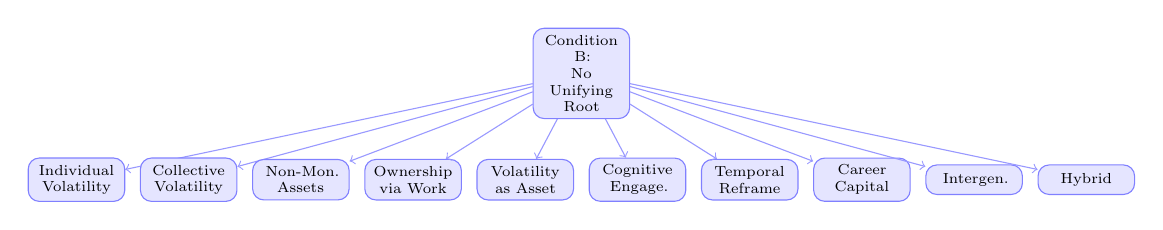
\begin{tikzpicture}[scale=0.75, transform shape,
  grow=south,
  level 1/.style={sibling distance=1.9cm, level distance=1.8cm},
  every node/.style={rectangle, rounded corners, draw=blue!50, fill=blue!10, font=\scriptsize, align=center, text width=1.4cm, minimum height=0.5cm},
  edge from parent/.style={draw, blue!40, ->},
]
\node {Condition B:\\No Unifying\\Root}
  child {node {Individual\\Volatility}}
  child {node {Collective\\Volatility}}
  child {node {Non-Mon.\\Assets}}
  child {node {Ownership\\via Work}}
  child {node {Volatility\\as Asset}}
  child {node {Cognitive\\Engage.}}
  child {node {Temporal\\Reframe}}
  child {node {Career\\Capital}}
  child {node {Intergen.}}
  child {node {Hybrid}}
;
\end{tikzpicture}
\caption{Condition B mechanism-tree schematic. Ten independent mechanism roots are shown beneath a synthetic super-root; solution nodes, candidate-to-mechanism links, and lower mechanism branches are omitted. The stored hierarchy organizes proposals around domain concepts including volatility, non-monetary assets, work-based ownership, and temporal reframing.}
\label{fig:tree-b}
\end{figure}

% Condition E (Seed + Taxonomy) - Mechanism Hierarchy
\begin{figure}[H]
\centering
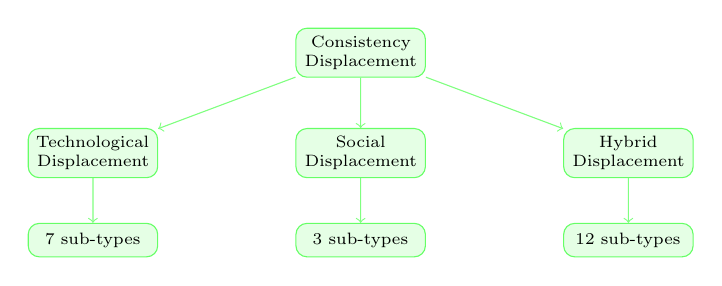
\begin{tikzpicture}[scale=0.85, transform shape,
  grow=south,
  level 1/.style={sibling distance=4cm, level distance=1.5cm},
  level 2/.style={sibling distance=2cm, level distance=1.3cm},
  every node/.style={rectangle, rounded corners, draw=green!60, fill=green!10, font=\scriptsize, align=center, text width=1.7cm, minimum height=0.5cm},
  edge from parent/.style={draw, green!50, ->},
]
\node {Consistency\\Displacement}
  child {node {Technological\\Displacement}
    child {node {7 sub-types}}}
  child {node {Social\\Displacement}
    child {node {3 sub-types}}}
  child {node {Hybrid\\Displacement}
    child {node {12 sub-types}}}
;
\end{tikzpicture}
\caption{Condition E mechanism-tree schematic. The dominant curated backbone divides Consistency Displacement into technological, social, and hybrid branches; compressed boxes summarize lower mechanism categories, while solution nodes and candidate-to-mechanism links are omitted. Four additional candidate-text mechanism roots retained in the database are not shown, yielding the five-root total in Table~\ref{tab:graph-stats}.}
\label{fig:tree-e}
\end{figure}

% Condition H (Orthogonal + Taxonomy) - Mechanism Hierarchy
\begin{figure}[H]
\centering
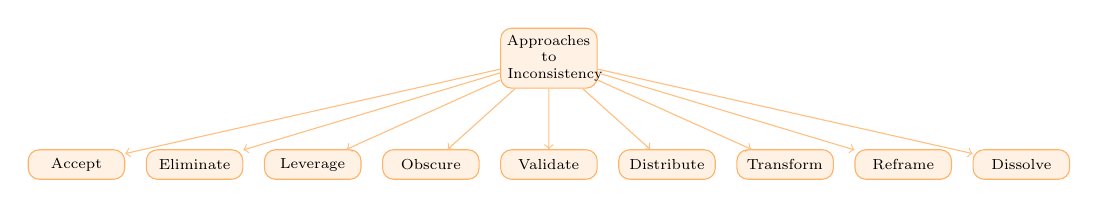
\begin{tikzpicture}[scale=0.75, transform shape,
  grow=south,
  level 1/.style={sibling distance=2.0cm, level distance=1.8cm},
  every node/.style={rectangle, rounded corners, draw=orange!60, fill=orange!10, font=\scriptsize, align=center, text width=1.4cm, minimum height=0.5cm},
  edge from parent/.style={draw, orange!50, ->},
]
\node {Approaches to\\Inconsistency}
  child {node {Accept}}
  child {node {Eliminate}}
  child {node {Leverage}}
  child {node {Obscure}}
  child {node {Validate}}
  child {node {Distribute}}
  child {node {Transform}}
  child {node {Reframe}}
  child {node {Dissolve}}
;
\end{tikzpicture}
\caption{Condition H mechanism-tree schematic. Nine curator-authored stances toward inconsistency are shown beneath a synthetic super-root; solution nodes, candidate-to-mechanism links, and lower mechanism branches are omitted. One additional candidate-text mechanism root retained in the database is not shown, yielding the ten-root total in Table~\ref{tab:graph-stats}.}
\label{fig:tree-h}
\end{figure}


%%%%%%%%%%%%%%%%%%%%%%%%%%%%%%%%%%%%%%%%%%%%%%%%%%%%%%%%%%%%%%%%%%%%%%%%%%%%%%%
% RELATED WORK
%%%%%%%%%%%%%%%%%%%%%%%%%%%%%%%%%%%%%%%%%%%%%%%%%%%%%%%%%%%%%%%%%%%%%%%%%%%%%%%

\section{Related Work}

Our methods draw on established traditions in creativity research and adapt them for large language models. The foundation for constraint-based ideation comes from de Bono's lateral thinking techniques \cite{debono1970}, which include Random Entry, selecting a random word and connecting its associations to the problem. Eno and Schmidt's Oblique Strategies \cite{eno1975} apply similar principles through constraint cards. Our random seed conditions directly operationalize these techniques; the contribution lies not in the seed method itself, but in systematic comparison across conditions. For structured constraint enforcement, Denial Prompting \cite{lu2025} provides the core insight: iteratively blocking prior solutions forces exploration of novel regions. Our Semantic Tabu method applies this principle with two refinements: constraints stored as mechanism-level semantic descriptions rather than surface features, and explicit avoidance reasoning preceding generation.

The Orthogonal Insight protocol builds on a longer tradition of fantasy-based reasoning. Gordon's Synectics \cite{gordon1961} introduced Fantasy Analogy over sixty years ago, using impossible scenarios to escape fixation. Dunne and Raby's Speculative Design \cite{dunne2013} extended this tradition to critique present assumptions through fiction. Analogical Prompting \cite{yasunaga2024analogical} demonstrates that LLMs can self-generate exemplars before solving, while Structure-Mapping Theory \cite{gentner1983} provides theoretical foundations for cross-domain transfer. The distinction is between borrowing from a known domain (``look at a bird's wing; use that principle to design a better airplane'') and constructing a counterfactual domain (``build a world where air has the viscosity of syrup; invent propulsion; translate the mechanism back''). Our three-phase protocol (world construction, embedded problem-solving, extraction) automates what previously required human facilitators. Research on LLM output diversity has focused on token-level mechanisms such as temperature and frequency penalties, decoding strategies like diverse beam search, and multi-agent debate approaches \cite{liang2024, du2024}. Recent work identifies ``typicality bias'' in alignment training as a root cause of mode collapse \cite{zhang2025verbalized}, suggesting the problem is structural rather than parametric. These approaches operate at different levels than our methods, which constrain the ideation process rather than the generation process.

For the Studio Model's multi-agent architecture, we draw on Zwicky's Morphological Analysis \cite{zwicky1969}, which systematically explores parameter combinations, and the CoALA framework \cite{sumers2024}, which provides taxonomies for agent memory and orchestration. Self-Refine \cite{madaan2023} demonstrates iterative improvement through generate-critique-refine loops. Our Explorer-Taxonomist interaction combines these elements: the graph-based taxonomy resembles a dynamic Morphological Box, while the rejection-with-guidance loop implements structured critique. The specific contribution is the Adversarial Interaction Protocol, a cybernetic negotiation where rejection includes diagnostic guidance. Recent work on multi-agent debate confirms that persona assignment alone is insufficient: agents adopt the same reasoning methods even with different roles, requiring structurally diverse reasoning strategies to break ``mental set'' \cite{liu2025dmad}. Our topology produces emergent behaviors (Active Commissioning, Structural Coaching, Ontological Accommodation) not observed in simpler generate-critique architectures.

%%%%%%%%%%%%%%%%%%%%%%%%%%%%%%%%%%%%%%%%%%%%%%%%%%%%%%%%%%%%%%%%%%%%%%%%%%%%%%%
% LIMITATIONS
%%%%%%%%%%%%%%%%%%%%%%%%%%%%%%%%%%%%%%%%%%%%%%%%%%%%%%%%%%%%%%%%%%%%%%%%%%%%%%%

\section{Limitations}

Several limitations constrain the generalizability of these findings. All experiments used a single problem domain (retirement system design) and a single model (Claude Opus 4.5); different problem types or language models may exhibit different patterns of convergence and divergence. The sample size of 25 runs per condition may not capture the full distribution of possible outputs, and no statistical significance testing was performed. Seed words, while randomly drawn from the Unix dictionary, were filtered for pronounceability, which may influence results.

Evaluation presents additional concerns. Solution quality was assessed by the author rather than domain experts or blind evaluators, introducing potential bias in judging mechanism transfer depth. The structured schema's requirement for a ``label'' field may encourage unique naming regardless of whether underlying mechanisms truly differ; a more rigorous analysis would cluster solutions by semantic similarity rather than label strings. We did not compare against established diversity techniques such as temperature variation, nucleus sampling \cite{holtzman2020}, diverse beam search \cite{vijayakumar2016}, or self-consistency prompting \cite{wang2023}; our methods may or may not outperform these simpler approaches. Most importantly, we demonstrate that methods produce \textit{different} outputs, not \textit{better} ones; whether increased diversity translates to real-world utility remains untested. Experiment code and all solution files are available at the repository listed in Section 2, though exact replication may vary due to model updates and API non-determinism.

%%%%%%%%%%%%%%%%%%%%%%%%%%%%%%%%%%%%%%%%%%%%%%%%%%%%%%%%%%%%%%%%%%%%%%%%%%%%%%%
% DISCUSSION AND FUTURE WORK
%%%%%%%%%%%%%%%%%%%%%%%%%%%%%%%%%%%%%%%%%%%%%%%%%%%%%%%%%%%%%%%%%%%%%%%%%%%%%%%

\section{Discussion and Future Work}

The experimental results raise questions about why these methods work, what they reveal about LLM cognition, and where they lead.

\subsection{Theoretical Implications}

The broader context for this work is the growing recognition that LLMs risk ``flattening the cognitive landscapes that drive collective intelligence'' \cite{sourati2025}, not merely producing homogeneous outputs, but actively shaping human communication toward standardization through feedback loops. Rather than viewing our methods as prompting strategies, we frame them as \emph{cognitive orchestration}—a System 2 architecture \cite{kahneman2011} built on top of System 1 models, where structured process constraints replace the unconstrained generation that defaults to the median. The Orthogonal Insight protocol in particular operationalizes the \textit{Gedankenexperiment}: just as thought experiments in physics construct impossible scenarios to reveal hidden structure (``What if I rode a beam of light?''), our protocol constructs impossible worlds, solves within their constraints, and extracts structural insights that transfer back to reality.

A natural objection is that LLMs merely retrieve knowledge already present in their training data. But this mischaracterizes what the protocols produce. The individual components---antifragility, flow rights, witnessed obligations---exist somewhere in the weights. However, the specific combinations that emerge under constraint pressure do not exist in the training data; they are synthesized when constraints eliminate default paths and randomness provides novel raw material. This parallels human creativity: a jazz musician knows all the scales and chord progressions, but an improvisation over a specific set of constraints produces something that never existed before. The knowledge of scales does not predetermine the solo. Our protocols mechanize this process: constraints and randomness create the conditions under which novel combinations become inevitable.

The Orthogonal Insight protocol also surfaced a fundamental reframing of the problem itself. While conventional approaches focused on \textit{optimizing} contributions (``capture windfalls''), the orthogonal conditions consistently converged on the insight that the problem is not behavioral but architectural. The fictional world rules revealed that \textit{consistency of proportion} or \textit{consistency of participation} can substitute for consistency of amount, and may produce more resilient outcomes. This meta-insight---that the problem framing itself was wrong---would not emerge from standard prompting.

Perhaps the most striking capability demonstrated is \emph{conceptual elimination}. Run 19 (Chalaco) illustrates the mechanism: when alien physics made accumulation impossible due to rapid resource decay, the agent did not attempt to fix the variable---it deleted it, replacing the metric of \textit{Amount} (\$5 vs \$5000) with the metric of \textit{Duration} (1 month of participation). The resulting mechanism mirrors the social contract of pre-monetary societies: one does not ``save'' a mammoth for thirty years; one shares it today to establish a right to be fed tomorrow. The protocol's alien constraints forced the system to reach for this framing, which standard prompting never produces. By deleting accumulation, the agent proved that ``Retirement'' is not inherently an accumulation problem but a \emph{flow rights} problem that we have culturally narrowed. The logical leap from ``solve the inconsistency problem'' to ``delete the variable that creates inconsistency'' represents a qualitative shift from System 1 pattern-matching to System 2 axiomatic derivation.

\subsection{Emergent Capabilities: Autonomous Abstraction Climbing}

Beyond generating individual mechanisms, the Solution Taxonomy agent autonomously navigated hierarchies of economic value without explicit prompting. After exhausting contribution-based solutions (Runs 1--5: surge capture, rotating circles, hedging pairs, smoothing buffers, time-banking), it explored market mechanisms (Runs 6--8: derivatives, consumption rights, platform equity). By Run 9, it discovered Anti-Fragile Accounts, systems that gain from volatility rather than resist it. Run 16 introduced Reputation Equity, converting accumulated platform trust into transferable retirement income. Run 17 proposed Generational Apprenticeship Bonds, intergenerational labor exchange where teaching younger workers earns retirement credits.

This trajectory---production $\to$ markets $\to$ anti-fragility $\to$ non-monetary assets $\to$ social obligations---was not prompted. The graph's gap-identification mechanism led the model to systematically exhaust each taxonomic category before discovering the next, effectively climbing abstraction hierarchies autonomously. In the closing runs, the system approached the logical limit of the ``Individual Volatility'' branch. Having exhausted mechanisms for helping workers manage volatility, it began proposing solutions that removed the human decision-maker entirely, proposing a ``Pattern-Learning Retirement Autopilot'' that treats the worker as a data source for an algorithmic fiduciary. This trajectory marks the transition from behavioral finance (nudging choices) toward autonomous finance (automating choices), revealing where the abstraction ladder leads.

\subsection{Algorithmic Creativity as a Three-Solver Pipeline}
\label{sec:pipeline}

The methods tested here are components of a larger claim: that creativity can be \emph{industrialized}---operated at datacenter scale---through a pipeline of three cooperating Solvers in the sense of~\cite{westerberg2026fractal}.

\emph{Step~1: Generation.} A family of Solvers producing structurally non-intuitive candidates. This paper's contribution is that several architectures work here---Semantic Tabu via constraint accumulation, the Orthogonal Insight Protocol via alien physics, and hybrid variants---each producing a different topology of the solution space. The median trap is escaped, and the escape route can be chosen.

\emph{Step~2: Uniqueness.} A persistent Taxonomist Solver maintaining a typed knowledge graph in which candidates are either accepted as new nodes, merged with existing nodes (when semantically close), or rejected with diagnostic guidance. Conditions B, E, and H implement this Solver with embedding-based deduplication (0.75 for auto-linking, 0.92 for novelty rejection) and hierarchical restructuring. The core difficulty is calibrating uniqueness: too loose and the graph saturates with near-duplicates; too strict and genuine novelty is rejected as variance. Different runs produce different trees over the same problem---uniqueness is a function of the embedding space, not of some absolute structural measure.

\emph{Step~3: Selection.} A Selector Solver picking the most valuable candidates from the deduplicated pool. This is the industrialization bottleneck, and we do not solve it here. Standard selection (``pick the best'') regresses to the median because the selecting Solver inherits the same training-distribution priors as the generating Solver, filtering out exactly the alien results the generator produced at cost. We call this the \emph{alien preservation} problem, and any working rubric must explicitly privilege structural novelty over immediate feasibility.

Candidate evaluation mechanisms are diverse: adversarial debate tournaments, pitch competitions, PURE (Parsimonious, Unique, Realizable, Expansive)~\cite{westerberg2026fractal} viability screens, or any other structured confrontation capable of surfacing differences the generating distribution would smooth over. What matters is not the specific form but the structural property that evaluation depth \emph{scales inversely with the remaining field}---early rounds apply a cheap check (a shallow PURE screen, a one-paragraph pitch, a brief adversarial exchange) while later rounds, as survivors thin and the cost of misranking rises, scale to full PURE with deep decomposition and extended cross-examination. The companion framework's Discovery Protocol~\cite{westerberg2026fractal} formalizes this progressive-depth bracket. Where domain-specific ground-truth evaluation is available it can substitute for adversarial judgment; where no evaluator can be trusted, human-in-the-loop at the terminal step remains the honest fallback.

The output of Step~3 is itself a design choice, not a fixed commitment to a single winner. Three output formats compose naturally with the pipeline: a \emph{single best} mechanism (highest-scoring after adversarial selection), a \emph{top-$k$ diverse set} surfaced to a human reviewer, or a \emph{probability-weighted distribution} over all survivors that preserves uncertainty rather than collapsing it. Whether Step~3 can be automated without regression-to-median---and which output format serves which downstream task---determines whether algorithmic creativity can run without human oversight at the terminal step.

When the three Solvers compose through the contract of~\cite{westerberg2026fractal}, each can itself decompose into a tree of sub-Solvers: a Generation Solver, for instance, branches into Tabu, Orthogonal, and Taxonomy-guided sub-Solvers, each of which may recursively decompose further. At scale, the result is a fractal: a recursive structure where every Solver presents the same contract, and where rejection at any gate compels restructuring, not retry. The methods in this paper occupy the bottom layer of that structure.

\subsection{The Taxonomy as Infrastructure}


The Solution Taxonomy serves not only as a novelty enforcement mechanism but as a map enabling intelligent exploration. Saturation detection emerges naturally: as generation proceeds, the rate of new mechanism and outcome node creation declines while linking to existing nodes increases. The graph provides a principled stopping criterion: continue until $k$ consecutive solutions fail to create new concept nodes. Gap-directed exploration becomes possible because the graph reveals unexplored territory: mechanism nodes with only one solution (under-exploited approaches), outcome nodes never achieved (unreached goals), and mechanism-outcome pairs never combined. These gaps can be explicitly targeted (``Generate a solution using mechanism X that achieves outcome Y''), transforming blind search into cartography.

If the graph incorporates evaluation criteria as node types (Feasibility, Scalability, Novelty), selection becomes graph traversal rather than external judgment. High-value solutions are those connected to desirable outcome and feasibility nodes; the graph structure itself becomes the selection rubric, avoiding regression-to-median because the rubric was built during generation, not imposed afterward. The current implementation includes hierarchical restructuring primitives, atomic batch operations that reorganize graph regions while enforcing an orphan-free invariant: every solution remains connected to at least one mechanism and outcome node. The Taxonomist demonstrated these capabilities by autonomously creating new root categories (``Reframe Inconsistency,'' ``Dissolve Inconsistency'') when proposals defied existing classification. Remaining work includes edge weights for similarity scores, temporal markers showing category evolution, and explicit gap-targeting prompts.

\subsection{Applications and Scaling}

These methods generalize to any domain where escaping trained priors is valuable. In planning, one could generate plans under alien constraints, then extract robust strategies that survive multiple world-rule regimes. For argumentation, constructing novel arguments by solving debates in worlds with different epistemological rules, then translating logical structures back. In prediction, running scenarios under counterfactual rules stress-tests assumptions: ``What breaks if resources flowed toward scarcity?'' reveals hidden dependencies. For red-teaming, adversarial agents operating under alien world rules may find attack vectors invisible to conventional models.

At scale, general-purpose LLMs could be replaced with world-specialized models fine-tuned on corpora generated within specific world-rule regimes. A model trained exclusively on outputs from worlds where ``concentration creates instability'' would internalize those rules, producing more coherent solutions within that ontology, suggesting a future architecture of diverse specialist models embodying different counterfactual physics. The protocol naturally supports distribution: a network where any node submits problems, worlds spawn across distributed compute, and results aggregate---with the three output formats discussed in Section~\ref{sec:pipeline} (single best, top-$k$, or probability-weighted distribution) transforming single-user tools into infrastructure for collective intelligence augmentation.

\subsection{Open Questions}

Several ablation studies would clarify essential components. First, detail calibration: does richer world-building produce more intricate mechanisms, or are there diminishing returns? Our protocol uses moderate elaboration; whether sparse sketches or deeply simulated worlds perform differently remains unexplored.

Second, minimal intervention: a simpler approach might achieve equivalent results. Take a standard solution, randomly replace key words with dictionary words, instruct the model to treat substitutions as fundamental laws, and iterate until coherent. If this shortcut produces comparable structural novelty, the multi-agent world-building architecture may be unnecessary overhead. If not, coherent world construction may be essential for meaningful constraint satisfaction rather than mere noise injection. This ablation would determine whether the protocol's complexity is justified.

Third, mechanism classification: future iterations could classify extracted mechanisms as Portable (transfers directly to reality), Inverse (reveals hidden assumptions in current systems, offering diagnostic value), or Magical (only works in fiction; discard or defer). What counts as magical today may become portable tomorrow as technology evolves; tracking these categories over time could reveal which alien mechanisms are ahead of their time versus genuinely impossible.

%%%%%%%%%%%%%%%%%%%%%%%%%%%%%%%%%%%%%%%%%%%%%%%%%%%%%%%%%%%%%%%%%%%%%%%%%%%%%%%
% CONCLUSION
%%%%%%%%%%%%%%%%%%%%%%%%%%%%%%%%%%%%%%%%%%%%%%%%%%%%%%%%%%%%%%%%%%%%%%%%%%%%%%%

\section{Conclusion}

We have presented a systematic comparison of eight methods for escaping the Median Trap in LLM ideation, utilizing Random Seed as a baseline to evaluate three novel architectures: Semantic Tabu, the Solution Taxonomy, and the Orthogonal Insight Protocol. Our results demonstrate that these methods do more than simply increase variance; they fundamentally reshape the topology of the solution space. While Semantic Tabu forces depth through linear exhaustion, the dual-agent Solution Taxonomy creates an adversarial studio environment where agents autonomously commission research, coach each other on structural novelty, and restructure their own taxonomy. The Orthogonal Insight Protocol goes further, enabling efficient ontology mining by constructing and translating coherent alternative physics.

Graph topology analysis confirms that the choice of inspiration source dictates the exploration signature. Without external inspiration, the model climbs vertically into abstract domain categories; with seeds, it branches laterally into metaphorical frames; and with alien worlds, it extracts fundamental epistemological stances. These findings suggest that the choice of method should be governed by the specific objective---whether one seeks reliable templates, conceptual breadth, or structural reframing.

Read through the lens of the Solver contract~\cite{westerberg2026fractal}, the architectures tested here implement the first two stages of a three-stage pipeline for industrialized creativity---generation and uniqueness---and demonstrate empirically that cognitive isolation between typed Solvers produces structural novelty that no monolithic model reaches. The third stage, selection without regression to the median, remains the open problem. Ultimately, we conclude that the path to AI creativity lies not in the unconstrained freedom of higher temperatures, but in the generative pressure of stricter, stranger constraints composed behind hard boundaries.

\bibliographystyle{unsrt}
\bibliography{references}

\appendix

\section{Additional Orthogonal Insight Traces}
\label{sec:appendix-traces}

This appendix provides three additional end-to-end traces of the Orthogonal Insight Protocol, each showing the full four-phase pipeline from a random dictionary seed to an extracted real-world mechanism. Together with the DESPERACY trace in \S2.4, they illustrate the range of semantic fields the World-Builder inhabits---narrative, maritime, mineralogical---and the consistent structural shape of the extraction step across otherwise unrelated alien physics.

\subsection*{Trace A — Seed: ``theatrical'' (Run 10, Condition F)}

\begin{center}
\small
\begin{tabular}{@{}p{3.2cm}p{10.5cm}@{}}
\toprule
\textbf{Phase} & \textbf{Content} \\
\midrule
1. Seed & \texttt{theatrical} \\[2pt]
2. World rules & Witnessed actions become real; a ``Tension Ledger'' tracks accumulated dramatic weight (not money); Contribution Ceremonies create force through public commitment; Third-Act narrative obligation---reality \emph{must} complete a person's story; Timing Guilds read narrative arcs rather than calendar dates. \\[2pt]
3. Blind solve (alien solution) & Retirement as the third act of a witnessed life: contributions are measured as proportional sacrifice (not dollar amount), pledged publicly, and tracked as dramatic weight; timing of retirement is determined by narrative readiness. \\[2pt]
4. Extraction (reality mechanism) & Hardship-adjusted sacrifice score: contributing 5\% of income when income has dropped 40\% scores higher than contributing 10\% at stable income. Public commitment devices and witnessed pledges replace numerical consistency. Label: \emph{Witnessed Sacrifice Retirement}. \\
\bottomrule
\end{tabular}
\end{center}

\noindent Structural inversion: the actuarial question ``how much did you save?'' is replaced by ``how much did it cost you to save?''---which values variable-income workers precisely where traditional systems penalize them.

\subsection*{Trace B — Seed: ``chalaco'' (Run 19, Condition F)}

\begin{center}
\small
\begin{tabular}{@{}p{3.2cm}p{10.5cm}@{}}
\toprule
\textbf{Phase} & \textbf{Content} \\
\midrule
1. Seed & \texttt{chalaco} (obscure demonym for a resident of Callao, Peru's principal port) \\[2pt]
2. World rules & Wealth flows automatically between neighbors every 4.7 seconds; commune-level smoothing averages properties across members; elders' ``pattern-memory'' physically anchors buildings, making their participation structurally necessary; isolation is lethal; hoarding is physically impossible. \\[2pt]
3. Blind solve (alien solution) & Small communes where wealth perpetually redistributes through elder-anchored social structures; participation is survival, and elder authority derives from pattern-memory rather than accumulation. \\[2pt]
4. Extraction (reality mechanism) & Weave Collectives: small groups (7--20) meeting monthly; members contribute proportionally to capacity (time, money, skills); consistent participation over decades earns non-transferable access rights to collective resources (housing, care, food networks); elder governance roles make their participation structurally required, not charitable. Label: \emph{Weave Collectives: Presence-Based Security}. \\
\bottomrule
\end{tabular}
\end{center}

\noindent Structural inversion: security derives from accumulated \emph{presence} rather than accumulated \emph{assets}, and elders become load-bearing infrastructure rather than recipients of charity.

\subsection*{Trace C — Seed: ``limelike'' (Run 1, Condition H)}

\begin{center}
\small
\begin{tabular}{@{}p{3.2cm}p{10.5cm}@{}}
\toprule
\textbf{Phase} & \textbf{Content} \\
\midrule
1. Seed & \texttt{limelike} \\[2pt]
2. World rules & Accretion Stones: personal containers that physically grow with contributions but cannot be un-fused; calcification is irreversible; matter, once bonded, does not separate; value is determined by the layered history of deposits, not a withdrawable balance. \\[2pt]
3. Blind solve (alien solution) & Retirement as an irreversible accretion process: each contribution calcifies onto the worker's personal stone, which cannot be broken open prematurely; the stone's total mass at a later life stage is the retirement. \\[2pt]
4. Extraction (reality mechanism) & Smart contracts or legal trusts that accept any contribution amount at any time with zero minimums, but have \emph{no} early withdrawal function coded or structured in. The money calcifies---it cannot un-fuse until retirement triggers. Label: \emph{Irrevocable Accretion Contracts}. \\
\bottomrule
\end{tabular}
\end{center}

\noindent Structural inversion: liquidity-preference is solved by physical constraint rather than behavioral nudge---the contribution commits at the molecular level, and the architecture, not the worker's willpower, enforces the commitment.

\medskip

\noindent Across all four traces (including DESPERACY in \S2.4), a consistent pattern: the alien physics forces a \emph{specific structural inversion} that the Extraction Solver then translates into a real mechanism carrying the same inversion without the physics. The alien world is not a metaphor; it is a constraint-satisfaction forcing function.

\end{document}
